\section{Andere Multi Layer Graph Systeme}

Im Folgendem werden verschiedene andere Systeme betrachtet, mit denen Multilayer Graphen analysiert werden können.

\subsection{MuxViz}

Das Analysetool MuxViz wurde von De Domenico, M. und Porter, M. A. und Arenas, A. in ihrer Arbeit ''MuxViz: a tool for multilayer analysis and visualization of networks vorgestellt'' \cite{De_Domenico_2014}.
MuxViz ist ein open-source Projekt, welches es ermöglicht Multi Layer Graphen mit verschiedenen Algorithmen zu analysieren und visualisieren. Es nutzt für die Berechnungen R sowie GNU Octave und bietet mit einem modularen Aufbau die Möglichkeit, das Nutzer eigene Funktionalität hinzufügen.


MuxViz bietet eine grafische Nutzeroberfläche, welche genutzt werden kann, um Graphen zu laden, Algorithmen auszuführen und Graphen sowie Ergebnisse zu visualisieren. Die Benutzeroberfläche ist Webbasiert, was ermöglicht, dass die tatsächlichen Berechnung entweder lokal oder auf einem entfernten Server durchgeführt werden.
Dabei gibt es eine große Auswahl an Algorithmen und Statistiken, die auf den Graphen angewandt werden können.


%\begin{figure}
%  \centering
%  \begin{subfigure}[b]{1.0\textwidth}
%    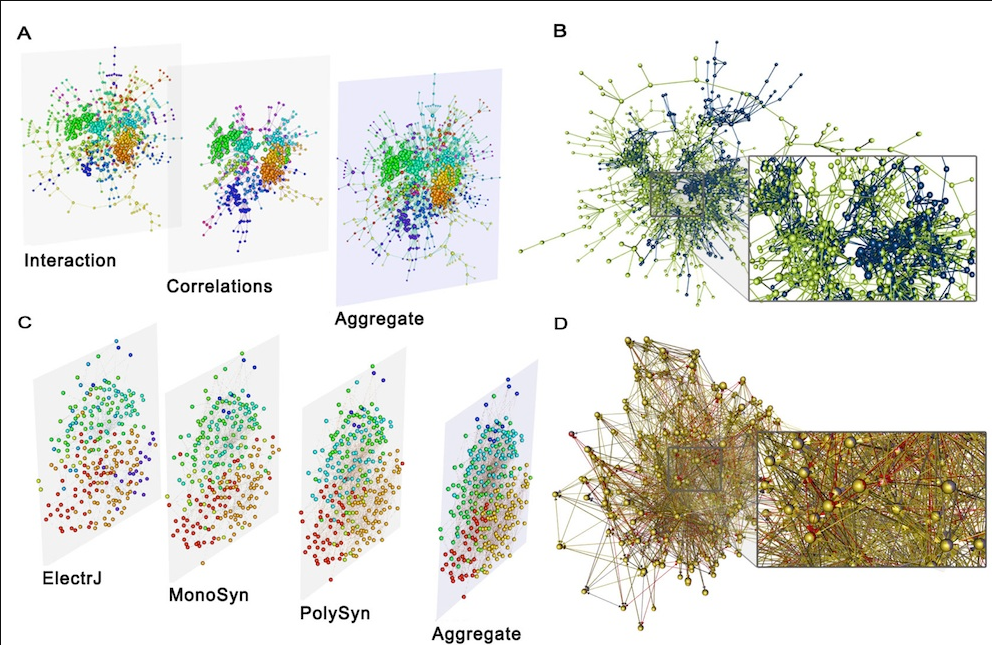
\includegraphics[width=1.0\linewidth]{img/muxViz.png}
%  \end{subfigure}
%  \caption{muxViz}
%  \label{muxVizSample}
%\end{figure}

\subsection{Multilayer Networks Library for Python}

Die Multilayer Networks Library for Python (Pymnet) wurde von Mikko Kivelä 2015 veröffentlicht. 
Die in Python geschriebene Bibliothek ermöglicht es mit Multilayer Netzwerke in Python zu arbeiten. Sie unterstützt das Laden und Manipulieren von Multilayer Netzwerken und bietet eine Reihe an Algorithmen zur Analyse der Netzwerke.
Zudem können Netzwerke mithilfe von Matplotlib und D3 visualisiert werden.
